\documentclass[timestamp,letterpaper,12pt,twoside]{uncthesis}

%%%%%%%%%%%%%%%%%%%%%%%%%%%%%%%%%%%%%%%%%%%%%%%%%%%%%%%%%%%%
% Required thesis information
%%%%%%%%%%%%%%%%%%%%%%%%%%%%%%%%%%%%%%%%%%%%%%%%%%%%%%%%%%%%

% When indicating your degree in the second bracketed space, use the full
% degree name (i.e., Doctor of Philosophy, not Ph.D. or PHD; Master of Public
% Health, not M.P.H. or MPH; Master of Social Work, not M.S.W. or MSW).
\uncdegreename{Master of Wizardry}

% List your department, school, or curriculum rather than your subject area or
% specialty discipline in the third bracketed space. You may include your
% subject area or specialty discipline in parentheses (i.e., Department of
% Romance Languages (French); School of Pharmacy (Molecular Pharmaceutics);
% School of Education (School Psychology); or similar official area).
% If you wish to include both your department and school names, list the school
% at the end of the statement (i.e., Department of Pharmacology in the School
% of Medicine).
% \uncthesisdepartment{Department of Pharmacology in the School of Medicine}
\uncthesisdepartment{House of Gryffindor}

% Type can be dissertation or thesis
\uncthesistype{thesis}

% Title
\uncthesistitle{Example Thesis}

% Name
\uncthesisauthor{Harry Potter}

% University Name
%\uncthesisuniversity{University of North Carolina at Chapel Hill}
\uncthesisuniversity{Hogwarts School of Witchcraft and Wizardry}

% The year in which your committee approves the completed thesis or
% dissertation. This need not be the year you graduate.
\uncthesisyear{1997}

% Thesis advisor. Appears on the abstract page.
\uncthesisadvisor{Albus Dumbledore}

% Thesis committee. Appears on the title page.  Do not include titles such as
% Professor, Doctor, Dr., PhD, or any identifiers such as “chair” or “advisor”
% before or after any names.  Put a new line after each name to render
% correctly on title page.
\uncthesiscommittee{Albus Dumbledore\\
Minerva McGonagall\\
Severus Snape\\
Remus Lupin\\
Rubeus Hagrid
}

%%%%%%%%%%%%%%%%%%%%%%%%%%%%%%%%%%%%%%%%%%%%%%%%%%%%%%%%%%%%
% Font selection
%%%%%%%%%%%%%%%%%%%%%%%%%%%%%%%%%%%%%%%%%%%%%%%%%%%%%%%%%%%%
% Font, if using PDFLaTeX
\usepackage{times}
% Font, if using XeLaTeX
%\usepackage{fontspec}
%\setmainfont{Times New Roman}

% Prevent awkward hyphenations.
\hyphenation{Raj-kumar}

\begin{document}
% The following order of the contents is REQUIRED
\pagenumbering{roman}

% 1. Title Page
\newgeometry{left=\uncthesisleftmargin in,top=2in,right=\uncthesisrightmargin in,bottom=1in,nohead}

\begin{titlepage}

\begin{singlespace}
\centering

\currentpdfbookmark{TITLE}{bk:title}

\vspace{1in}
\begin{adjustwidth}{0.5in}{0.5in}
\centering
\MakeUppercase{\uncthesistitle}
\end{adjustwidth}

\nointerlineskip\vspace{1in}

\uncthesisauthor{}

\nointerlineskip\vspace{1in}

\noindent
A \uncthesistype{} submitted to the faculty at the \uncthesisuniversity{} in partial fulfillment of the requirements for the degree of \uncdegreename{} in the \uncthesisdepartment{}.

\nointerlineskip\vspace{1in}

Chapel Hill\\
\uncthesisyear{}
%\the\year

\end{singlespace}

% Use the following block if you want the committee members to have exactly a 1in margin to the right.
%\nointerlineskip\vspace{0.83in}
%\setlength\topsep{0pt}
%\begin{flushright}
%{
%\setlength{\tabcolsep}{0pt}
%\begin{tabular}[t]{l}
%Approved by: \\
%\thesismembers
%\end{tabular}
%} % large
%\end{flushright}

% Use the following block if you want the committee members to appear approximately 2/3 the way across the page.
\nointerlineskip\vspace{0.71in}
\begin{flushright}
\begin{minipage}{2.1in}
\setlength{\tabcolsep}{0em}
\begin{tabular}{l}
Approved by: \\
\uncthesiscommittee{}
\end{tabular}
\end{minipage}
\end{flushright}

\end{titlepage}


% 2. Copyright Page (optional)
\newgeometry{left=\uncthesisleftmargin in,top=8.42in,right=\uncthesisrightmargin in,bottom=1in,nohead}

\begin{center}
\begin{singlespace}
\copyright~\uncthesisyear\\
\uncthesisauthor \\
ALL RIGHTS RESERVED
\end{singlespace}
\end{center}

\clearpage
\newgeometry{left=\uncthesisleftmargin in,top=2in,right=\uncthesisrightmargin in,bottom=1in,nohead}
% Normal pages from here on out; TOC title takes care of 2in requirement.
\restoregeometry


% 3. Abstract
\begin{abstract}

Abstracts cannot exceed 150 words for a thesis or 350 words for a dissertation.

\lipsum

\end{abstract}


% 4. Dedication, Acknowledgement(s), Preface (each optional)
\begin{dedication}
A dedication is a message from the author prefixed to a work in tribute to a person, group, or cause. Most dedications are short statements of tribute beginning with \textit{``To \ldots''} such as \textit{``To my family''}.
\end{dedication}

\begin{acknowledgement}

Acknowledgements are the author's statement of gratitude to and recognition of the people and institutions that helped the author's research and writing.

    \lipsum[5]
\end{acknowledgement}

\begin{preface}

A preface is a statement of the author's reasons for undertaking the work and other personal comments that are not directly germane to the materials presented in other sections of the thesis or dissertation. These reasons tend to be of a personal nature.

    \lipsum[6]

\end{preface}


% 5. Table of Contents, with page references
\renewcommand{\contentsname}{\hfill\bfseries\normalsize TABLE OF CONTENTS\hfill}
%\renewcommand{\cfttoctitlefont}{\hfill\Large\bfseries}
\renewcommand{\cftaftertoctitle}{\hfill}
\renewcommand{\cftdotsep}{1.5}
\cftsetrmarg{1.0in}

\setlength{\cftbeforetoctitleskip}{56pt}
\setlength{\cftaftertoctitleskip}{18pt}

% format chapter entries like other entries
\renewcommand{\cftchapfont}{\normalfont}
\renewcommand{\cftchappagefont}{\normalfont}
\renewcommand{\cftchapleader}{\cftdotfill{\cftdotsep}}

\setlength{\cftbeforechapskip}{15pt}
\setlength{\cftbeforesecskip}{10pt}
\setlength{\cftbeforesubsecskip}{10pt}
\setlength{\cftbeforesubsubsecskip}{10pt}

\begin{singlespace}
\currentpdfbookmark{TABLE OF CONTENTS}{bk:contents}
\tableofcontents
\end{singlespace}

\clearpage


% 6. List of Tables, with titles and page references (if applicable). And list
% of Figures or Illustrations, with titles and page references (if applicable)
\renewcommand{\listtablename}{LIST OF TABLES}
\phantomsection
\addcontentsline{toc}{chapter}{LIST OF TABLES}

\setlength{\cftbeforelottitleskip}{-14pt}
\setlength{\cftafterlottitleskip}{22pt}
\renewcommand{\cftlottitlefont}{\hfill\normalsize\bfseries}
\renewcommand{\cftafterlottitle}{\hfill}

\setlength{\cftbeforetabskip}{12pt}
\cftsetrmarg{1.0in}

\setlength{\cfttabindent}{0in}

\begin{singlespace}
\listoftables
\end{singlespace}

\clearpage

\renewcommand{\listfigurename}{LIST OF FIGURES}
\phantomsection
\addcontentsline{toc}{chapter}{LIST OF FIGURES}

\setlength{\cftbeforeloftitleskip}{-14pt}
\setlength{\cftafterloftitleskip}{22pt}
\renewcommand{\cftloftitlefont}{\hfill\normalsize\bfseries}
\renewcommand{\cftafterloftitle}{\hfill}

\setlength{\cftbeforefigskip}{12pt}
\cftsetrmarg{1.0in}

\setlength{\cftfigindent}{0in}

\begin{singlespace}
\listoffigures
\end{singlespace}

\clearpage


% 7. List of Abbreviations (if applicable)
\phantomsection
\addcontentsline{toc}{chapter}{LIST OF ABBREVIATIONS}

\begin{center}
\textbf{LIST OF ABBREVIATIONS}
\vspace{16pt}
\end{center}

% TODO: define new column types to make sure multi-line table cells has single-spacing

\noindent
\begin{tabular}{p{0.8in} p{5in}}
CoS     & Chamber of Secrets\\
DA      & Dumbledore's Army\\
DADA    & Defence Against the Dark Arts\\
DH      & Deathly Hallows \\
FBAWTFT & Fantastic Beasts and Where to Find Them\\
SPEW    & Society for the Protection of Elvish Welfare\\
VWI     & Voldemort War One\\
VWII    & Voldemort War Two\\
\end{tabular}

\clearpage


% 8. List of Symbols (if applicable)
\phantomsection{}
\addcontentsline{toc}{chapter}{LIST OF SYMBOLS}

\begin{center}
\textbf{LIST OF SYMBOLS}
\vspace{16pt}
\end{center}

\noindent
\begin{tabular}{@{}p{0.8in} l}
$M$ & Number of wands\\
$m$ & Number of wizards\\
$n$ & Number of fantastic beasts\\
\end{tabular}

\clearpage


\pagenumbering{arabic}

\chapter{Formatting Guide}
\label{chap:formatting_guide}

\section{Margins}

This template follows the UNC graduate school thesis/dissertation formatting guide as rigidly as possible.
This template has uniform margins throughout the entire document:
\begin{itemize}
    \item Left: 1''
    \item Right: 1''
    \item Top: 1''
    \item Bottom: 1''
\end{itemize}

\section{Font}
A TrueType font is recommended/required by the ProQuest dissertation publishing. Recommended fonts and sizes can be found in \autoref{tab:font}.

\begin{table}
    \centering
    \caption{Recommended font type and size}\label{tab:font}
    \begin{tabular}{ll}
        \toprule
        Font name            & Font Size \\ \midrule
        Arial                & 10pt\\
        Century              & 11pt\\
        Courier New          & 10pt\\
        Garamond             & 12pt\\
        Georgia              & 11pt\\
        Lucida Bright        & 10pt\\
        Microsoft Sans Serif & 10pt\\
        Tahoma               & 10pt\\
        Times New Roman      & 12pt\\
        Trebuchet MS         & 10pt\\
        Verdana              & 10pt\\ \bottomrule
    \end{tabular}
\end{table}

If you're using \texttt{pdflatex} to compile this template, include the \texttt{times} package in the preamble.
If you're using \texttt{xelatex} to compile this template, you can use the \texttt{fontspec} package and the \texttt{setmainfont} command to choose your favorite font.
This template by default uses 12pt Times New Roman.

\section{Spacing and Indentation}

The template takes care of spacing and indentation:
\begin{itemize}
    \item Text appears in a single column on each page and is double-spaced throughout the document.
    \item New paragraphs are indicated by a consistent tab indentation throughout the entire document.
    \item The document text is left-justified.
    \item For blocked quotations, indent the entire text of the quotation consistently from the left margin.
\end{itemize}

\lipsum[6]
\begin{quote}
    This is an example showing the indentation of block quoted text.
    \lipsum[8]
\end{quote}
\lipsum[7]

\section{Pagination}
This template takes care of pagination.

Pagination and margin are also well maintained for landscape pages.
\begin{landscape}
    \lipsum[9] Let's also see how does footnote works in landscape pages~\footnote{We have a footnote in landscape environment}.
\end{landscape}

\section{Footnotes and Endnotes}
Footnotes\footnote{\lipsum[10]} and endnotes\footnote{\lipsum[11]} obey the
formatting guide. However, using both of them confuses the note numbering.
Given the discrepancy between the official format guide\endnote{\lipsum[12]}
and the official sample pages\endnote{\lipsum[14]}, the correct order for
endnotes and appendixes are unclear.  Thus, using only footnote is recommended.

\section{Tables and Figures}
Tables, figures, and illustrations vary widely by discipline. Therefore, formatting of these
components is largely at the discretion of the author.

List of figures and list of tables are well taken care of by \LaTeX{} and this
template.  If an entry in LOT/LOF takes up more than one line, break up the
entry about three-fourths of the way across the page and place the rest of the
text on a second line, single-spacing the two lines.

One nice trick is the short caption option for the
\texttt{\textbackslash{}caption{}} command.  It allows the LOT/LOF only include
the short caption but not the full caption.
\begin{figure}
    \centering
    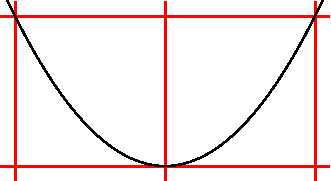
\includegraphics[width=0.5\textwidth]{figures/demo.pdf}
    \caption{A very long caption that does not make much sense but only tests the line-breaking and line-spacing in LOT/LOF.}
\end{figure}

\begin{figure}
    \centering
    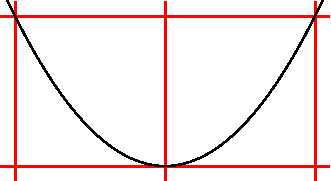
\includegraphics[width=0.5\textwidth]{figures/demo.pdf}
    \caption[Short Caption]{A very long caption that does not make much sense but only tests the line-breaking and line-spacing in LOT/LOF.}
\end{figure}

\section{Reference}
The APA style is used for references. Notice the differences caused by different citation command.

\begin{table}
    \centering
    \caption[Short title]{Comparison of different citation command.}\label{tab:citation}
    \begin{tabular}{ll}
        \toprule
Command                        & Results \\ \midrule
\texttt{\textbackslash{}cite}  & \cite{LFR}\\
\texttt{\textbackslash{}citep} & \citep{LFR}\\
\texttt{\textbackslash{}citet} & \citet{LFR}\\\bottomrule
    \end{tabular}
\end{table}

\section{Length}
There are no requirements for the length of the PhD thesis. For the Department of Computer Science, from 2014 to 2017, average length of the thesis main body text is $\mu \approx 120, \sigma \approx 33$, average length of main body text + reference is $\mu \approx 129, \sigma \approx 35$.
\chapter{Related Works}
\label{chap:related}

\section{A very long section title testing the line-breaking and line-spacing in TOC if not long enough we make it longer}
\subsection{Subsection title}
\lipsum{}
\subsubsection{Subsubsection title}
\lipsum[1]
\subsection{Another subsection title}


% The graduate school Format Guide put endnotes before appendixes But the
% provided sample pages put appendixes before endnotes It's unclear which one
% is correct. Recommend to use footnotes instead of endnotes.
\appendix
\chapter{Example Appendix}
\label{chap:appendix}
\lipsum[1]

\chapter{Another Appendix}
\label{chap:appendix2}

\lipsum[1]

\clearpage

\begin{center}
\vspace*{46pt}
\currentpdfbookmark{ENDNOTES}{bk:endnotes}
\textbf{ENDNOTES}
\vspace{10pt}
\end{center}
\addcontentsline{toc}{chapter}{ENDNOTES}

\theendnotes{}

\clearpage


\clearpage
\phantomsection

{\def\chapter*#1{} % suppress bibliograph header.
\begin{singlespace}
\addcontentsline{toc}{chapter}{REFERENCES}
\begin{center}
\textbf{REFERENCES}
\vspace{17pt}
\end{center}

\bibliographystyle{apalike}
\bibliography{references}
\end{singlespace}
}

\end{document}
